% ============================================================================================================
\chapter{Validation empirique}\label{ch:validation}
% ============================================================================================================

La validation a trois volets : la disparition du paradoxe qui a motivé la réforme, la confrontation de quelques
résultats à des évaluations empiriques indépendantes, et des tests automatisés de cohérence comportementale.

\section{Les chocs d'offre ont désormais le bon signe}

\begin{table}[h]\centering\small
\caption{Chocs d'offre défavorables dans la v0.6 et la v0.7 (écarts à la référence en 2037). Simulations exécutées
(\code{phase3/diagnostic\_fermeture.py}).}\label{tab:diag}
\tabfit{../tables/diagnostic.tex}
\end{table}

Avec la v0.7, le ralentissement de la productivité réduit le PIB de 3,2 \% en 2037 (le PIB potentiel baisse de
3,3 \%), le chômage remonte de 0,4 point et la dette augmente de 1,8 point de PIB en 2037 et d'une vingtaine de points
en 2047 (figure~\ref{fig:diagprod}). Le choc démographique réduit le PIB de 1,4 \% et augmente la dette d'un point. Les
premières années, la dette baisse encore légèrement : la hausse des coûts unitaires fait monter les prix, donc le PIB
nominal ; cet effet d'inflation s'épuise ensuite. Sans fermeture ($\rho = 0$), le paradoxe réapparaît (dette $-16$
points en 2037) : c'est bien le bloc d'offre qui corrige le défaut.

\begin{figure}[htbp]\centering
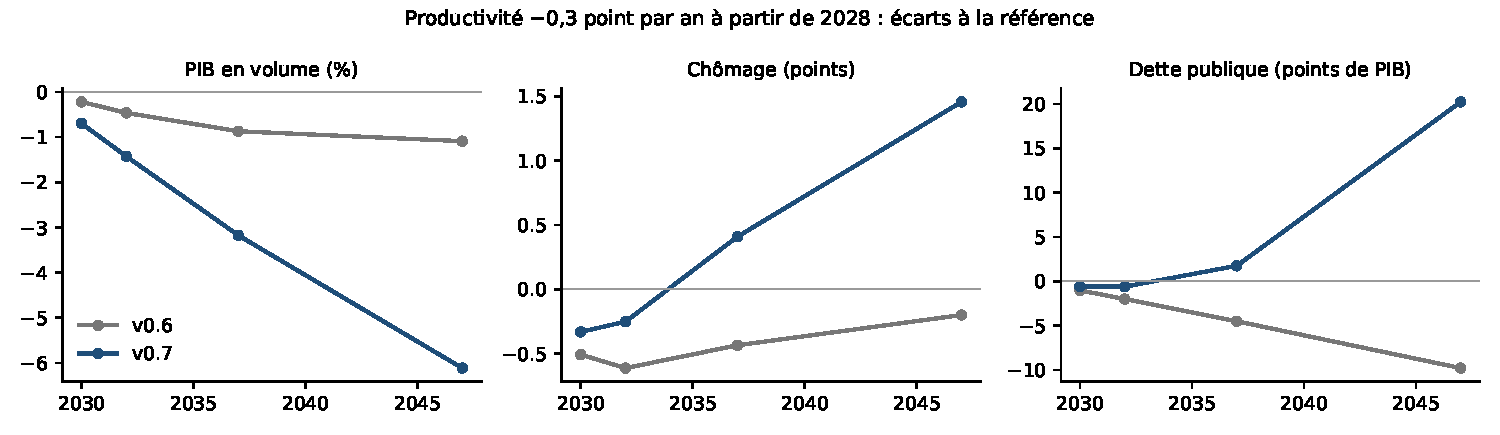
\includegraphics[width=\linewidth]{diagnostic_productivite.pdf}
\caption{Choc de productivité : trajectoires comparées v0.6 et v0.7.}\label{fig:diagprod}
\end{figure}

Le choc démographique fait baisser le chômage de 0,5 point en 2037 : la population active diminue plus vite que
l'emploi, ce qui crée des tensions sur le marché du travail et fait monter les salaires (+1,4 \%). Ce résultat est
cohérent avec la situation de pénurie de main-d'œuvre ; il se résorbe lentement, par les salaires.

\section{Confrontation à des évaluations indépendantes}

\paragraph{Baisse du coût du travail (CICE).} Le CICE, d'environ 20\md, a créé de l'ordre de 100 000 emplois selon
l'évaluation de France Stratégie (2020), 160 000 dans l'estimation macroéconomique. La v0.7 donne, pour une baisse de
cotisations employeurs de 20\md, $+129\,000$ emplois en 2030, $+157\,000$ en 2032 et $+122\,000$ en 2037 (v0.6 :
$+105\,000$, $+109\,000$ et $+53\,000$). L'ordre de grandeur est conforme ; la v0.7 rend l'effet plus durable, parce
que la baisse du coût du travail augmente la production potentielle.

\paragraph{TVA.} Une hausse d'un point du taux normal augmente les prix à la consommation de 0,54 \% après un an,
une baisse les réduit de 0,28 \% seulement ; pour les taux réduits, +0,40 \% contre $-0{,}20$ \%. L'asymétrie
documentée par Benzarti et al. (2020) est reproduite par construction ; l'intérêt est d'en voir les conséquences :
une baisse de TVA coûte presque autant aux finances publiques qu'une hausse en rapporte (2,4 points de dette en 2037
pour $-1$ point de TVA), mais soutient beaucoup moins le pouvoir d'achat, une partie allant aux marges.

\paragraph{Impôt sur les sociétés.} Une baisse du taux à 20 \% augmente l'investissement des entreprises de 0,87 \%
en 2032 (0,75 \% avec le comportement bas, 1,10 \% avec le haut), essentiellement par le coût d'usage du capital de
l'équation estimée. L'effet est modeste au regard du coût budgétaire (+4,7 points de dette en 2037), ce qui est
cohérent avec l'absence d'effet concluant du CICE sur l'investissement et avec les travaux sur la réforme des
dividendes de 2013. Une hausse à 28 \% rapporte moins qu'en v0.6, du fait du transfert de bénéfices.

\paragraph{Offre de travail.} Une hausse de 25 \% du RSA réduit la population active de 60 000 personnes (personnes
seules, parents isolés, couples dont aucun membre ne travaille) ; une hausse de 25 \% de la prime d'activité
l'augmente de 101 000. La baisse de 10 \% des aides au logement augmente la population active de 72 000 personnes, la
hausse d'un point de CSG la réduit de 39 000. Ces ordres de grandeur sont dans le haut de ce que suggèrent les
évaluations françaises des incitations financières à l'emploi, qui trouvent des effets de participation réels mais
modestes ; ils sont donc présentés avec la fourchette basse (élasticité 0,1) et haute (0,4).

\section{Tests automatisés}

Le fichier \code{tests/test\_phase3.py} contient douze tests qui vérifient, sur des simulations exécutées, des
propriétés attendues par la théorie ou la littérature : la référence est identique sous les deux fermetures ; un choc
de productivité réduit le PIB et augmente la dette à long terme ; un choc démographique réduit le PIB ; une hausse
des taux réduit l'investissement et le PIB et augmente la dette ; un supplément de demande augmente d'abord la
production puis les prix ; la TVA est asymétrique ; une baisse d'IS n'augmente l'investissement que faiblement ;
une hausse d'IS rapporte moins quand le transfert de bénéfices est plus fort ; le RSA et la prime d'activité ont des
effets de sens opposé sur la participation ; les réactions diffèrent selon la configuration familiale ; les niveaux
bas, central et haut sont ordonnés. Résultat de l'exécution : 12 tests sur 12 réussis (exécution du 23 novembre 2026, 14 minutes, \code{python3 -m pytest tests/test\_phase3.py}).


\begin{limites}[Ce qui n'a pas été validé]
Les nouveaux paramètres sont calibrés, pas estimés. La v0.7 n'a pas fait l'objet d'un test rétrospectif complet
(simulation de 2010-2025 avec les seules données disponibles à chaque date) : les équations estimées sont celles de la
v0.6, déjà testées hors échantillon, mais l'effet des nouveaux termes sur la qualité de l'ajustement historique n'a
pas été mesuré.
\end{limites}

% ============================================================================================================
\chapter{Comparaison avec la version 0.6}\label{ch:comparaison}
% ============================================================================================================

Toutes les expériences du rapport v0.6 ont été relancées avec la v0.7 (68 simulations, dont 10 nouvelles). Le fichier
\code{comparaison\_v06\_v07.xlsx} donne, pour chacune, seize indicateurs (consommation, investissement, exportations,
importations, emploi, chômage, salaires, prix, revenu disponible réel, épargne, recettes, dépenses, solde, dette,
industrie) à 5, 10 et 20 ans. Le tableau~\ref{tab:comp} en extrait l'essentiel.

\begin{table}[htbp]\centering\scriptsize
\caption{Principales mesures : effets en 2037 dans la v0.6 et la v0.7 (PIB en \%, emploi en milliers, chômage et dette
en points).}\label{tab:comp}
\tabfit{../tables/comparaison.tex}
\end{table}

\begin{figure}[htbp]\centering
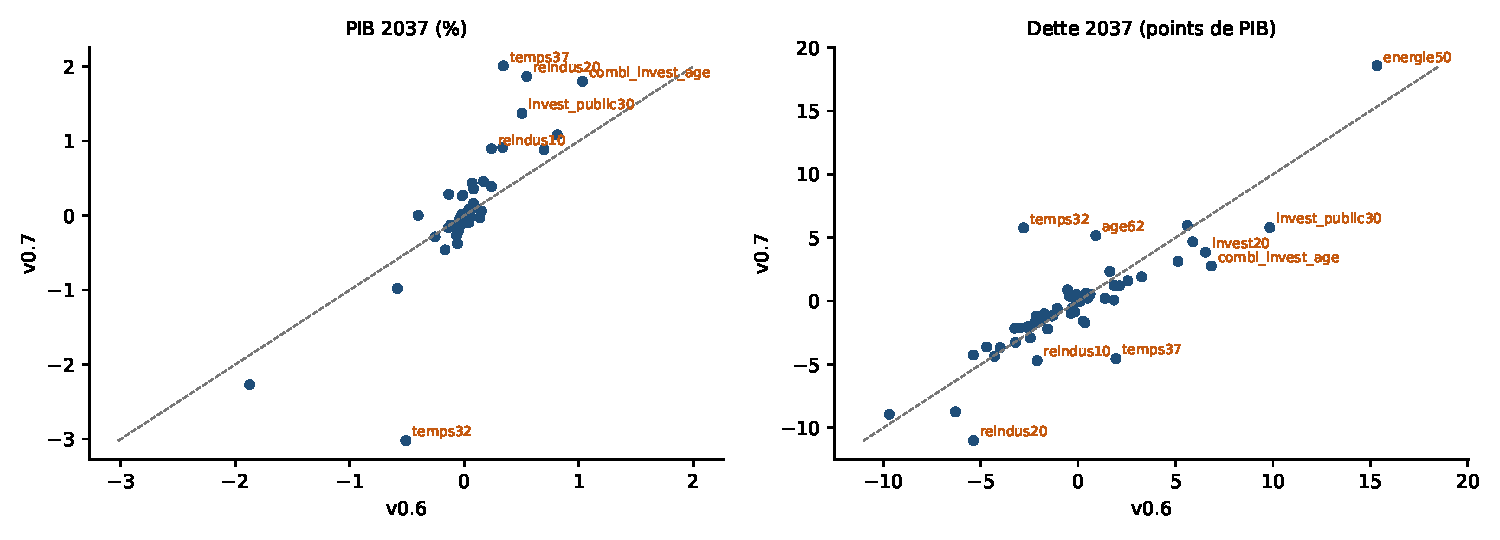
\includegraphics[width=\linewidth]{comparaison_v06_v07.pdf}
\caption{Chaque point est une expérience : effet en 2037 dans la v0.6 (abscisse) et dans la v0.7 (ordonnée). Les
mesures dont l'effet change le plus sont nommées.}\label{fig:comp}
\end{figure}

\section{Ce qui change, et pourquoi}

\begin{enumerate}
\item \textbf{Les mesures d'offre ont des effets plus forts et plus durables.} Relever l'âge légal à 65 ans augmente le
PIB de 0,9 \% en 2037 et réduit la dette de 1,6 point (en v0.6 : +0,7 \% et +0,3 point de dette : la hausse de la
population active ne trouvait pas d'emploi faute de demande). Revenir à 62 ans coûte 2,3 points de PIB et 5,2 points
de dette (v0.6 : 1,9 point de PIB et 0,9 point de dette). Les mesures qui allongent la durée du travail ont des
effets beaucoup plus grands qu'en v0.6, mais reposent sur une hypothèse non estimée (chapitre~\ref{ch:limites}).
\item \textbf{Les mesures de demande s'estompent.} Les effets des dépenses publiques et des transferts diminuent avec
le temps, parce que la production revient vers le potentiel. L'investissement public garde un effet durable, parce
qu'il augmente le capital et donc le potentiel.
\item \textbf{Les prestations ont désormais des effets d'offre.} La prime d'activité augmente la population active ;
le RSA la réduit légèrement ; les aides au logement ont un effet de taux marginal. En v0.6, RSA et prime d'activité
n'étaient que des transferts.
\item \textbf{Les impôts sur les entreprises rapportent moins.} La hausse de l'IS rapporte 40 \% de moins en 2037
(transfert de bénéfices) ; la baisse coûte aussi moins.
\item \textbf{Les baisses de TVA sont moins efficaces pour le pouvoir d'achat}, à coût budgétaire presque identique.
\item \textbf{Les chocs énergétiques sont plus coûteux} : le prix de l'énergie importée +50 \% augmente le chômage de
1,3 point en 2037 (0,6 en v0.6) et la dette de 18,6 points (15,4).
\end{enumerate}

\begin{resultat}
Les conclusions qualitatives de la v0.6 sur les mesures fiscales et budgétaires sont, pour l'essentiel, confirmées ;
celles qui concernent les réformes d'offre (âge de départ, durée du travail, offre de travail) changent nettement,
parce que la v0.6 ne pouvait pas les représenter correctement.
\end{resultat}

% ============================================================================================================
\chapter{Interactions entre comportements et sous-modèles}\label{ch:interactions}
% ============================================================================================================

\section{Sensibilité aux comportements}

Le tableau~\ref{tab:comport} montre, pour dix mesures, les résultats avec les trois niveaux de comportement. La
plupart des mesures fiscales et budgétaires sont peu sensibles aux paramètres comportementaux de la phase 3 : leurs
effets passent surtout par les équations estimées. Trois familles le sont nettement plus :
\begin{itemize}
\item la R\&D, dont l'effet sur le PIB varie de 0,07 \% à 1,44 \% en 2037 selon l'additionnalité et le rendement du stock
de R\&D : c'est le levier dont la conclusion dépend le plus des hypothèses ;
\item les prestations liées à l'emploi (prime d'activité, RSA), via l'élasticité de participation ;
\item les chocs d'énergie, via la délocalisation des industries énergo-intensives et l'épargne de précaution.
\end{itemize}

\begin{table}[htbp]\centering\scriptsize
\caption{Effets en 2037 selon le niveau des comportements (bas, central, haut).}\label{tab:comport}
\tabfit{../tables/comportements.tex}
\end{table}

\section{Interactions avec les sous-modèles}

\paragraph{Microsimulation (M10) et offre de travail (M15).} Les mesures de prélèvements et de prestations passent
par OpenFisca deux fois : pour les revenus (effet statique sur le revenu disponible des ménages, par décile et par
groupe) et pour les incitations (gain à l'emploi et taux marginal par configuration familiale). Les deux calculs
utilisent la même législation et les mêmes barèmes, ce qui évite les incohérences, mais pas les mêmes populations :
M10 utilise l'échantillon de ménages, M15 des cas types pondérés par le recensement.

\paragraph{Retraites (M9).} Le relèvement de l'âge légal modifie la population active de seniors ; dans la v0.7,
cette population active supplémentaire augmente le PIB potentiel, et la fermeture fait progressivement monter la
demande à son niveau. C'est le principal changement de conclusion par rapport à la v0.6.

\paragraph{Zone euro (M11).} Les simulations de programmes incluent la rétroaction de la zone euro (demande
européenne, taux). Elle est d'un ordre de grandeur inférieur aux effets domestiques.

\paragraph{Hauts revenus (M13) et hétérogénéité (M14).} Inchangés ; ils interagissent avec la v0.7 par le revenu
disponible (consommation) et par les dividendes (le canal de trésorerie des entreprises s'ajoute à la distribution
des profits de M14).

\paragraph{Anticipation.} Le terme d'anticipation transmet à la demande toute révision du potentiel, y compris celles
qui viennent des mesures (âge légal, offre de travail, R\&D). Son intensité a été testée sur les stratégies
(chapitre~\ref{ch:robustesse}).
